
The C ORB Interface System (CORBin) consists of two components: an IDL compiler, 
corbin-idl,  and a library of C functions.   The sections in this chapter 
discuss these two parts of the C ORB Interface system in detail. 

\section*{\underline{The IDL Compiler:  corbin-idl}}
\addcontentsline{toc}{section}{The IDL Compiler:  corbin-idl}

The corbin-idl compiler, like any IDL compiler, is used to produce stubs and 
skeletons from an IDL specification.   Corbin-idl parses IDL specifications
according the the IDL grammar found in the CORBA 2$.$4 specification.
Since corbin-idl relies upon ORBit to do the actual marshalling and 
de-marshalling of parameters for operation invocations on CORBA objects, 
corbin-idl generates C functions that {\em{wrap}} the functions generated 
by orbit-idl, the IDL compiler for ORBit.   In addition to generating 
C code, corbin-idl generates ML code that works with the SML/NJ C 
interface. \cite{lorenz} This ML code must be explicitly loaded into 
the top-level environment of SML/NJ before CORBin related functions 
may be used. The subsections that follow discuss the process of 
stub and skeleton generation for the C ORB Interface. 

\subsection*{IDL stubs}
\addcontentsline{toc}{subsection}{IDL stubs} 

There are four key steps involved in the corbin-idl stub generation process.
Since corbin-idl acts as an interface to ORBit, the first step in this 
process is to generate C functions that wrap the IDL stub functions generated 
by ORBit's IDL compiler, orbit-idl.   
Suppose the IDL specification defined in figure \ref{foointerface} 
is given as input to corbin-idl.
\begin{figure*}[t]
\singlespace
\begin{verbatim}

     interface foo {

          long bar(in long x); 

     };

\end{verbatim}
\doublespace
\caption {\em {IDL Specification for a CORBA object called foo}.}
\figline
        \label{foointerface}
\end{figure*}
Once corbin-idl has parsed this IDL specification, it generates a 
C function to wrap the stub function for the bar operation. 
This C function is illustrated in figure \ref{CStubWrapper}.
\begin{figure*}[t]
\singlespace
\begin{verbatim}

     long CORBin_foo_bar(CORBA_Object obj, long x)
     {
          return foo_bar(obj, x, &ev);
     }
 
\end{verbatim}
\doublespace
\caption {\em {C function generated by corbin-idl to invoke the bar operation of a foo object}.}
\figline
        \label{CStubWrapper}
\end{figure*}

Because CORBin utilizes the SML/NJ C foreign function interface, 
corbin-idl must generate C macros to explicitly define the stub function 
wrappers in the SML/NJ runtime system.
The C Macro generated for the CORBin\_foo\_bar function 
is shown in figure \ref{CStubMacro}.
This macro is appended to a C header file that is included during the 
building process of the SML/NJ runtime system.  This is done so that the 
CORBin\_foo\_bar function can be made available to the ML programmer
in the top-level environment of SML/NJ.
\begin{figure*}[t]
\singlespace
\begin{verbatim}

C_CALLS_CFUNC("CORBin_foo_bar",CORBin_foo_bar,long ,(void *, long ))
 
\end{verbatim}
\doublespace
\caption {\em {C Macro to explicitly define the CORBin\_foo\_bar function in the SML/NJ runtime system}.}
\figline
        \label{CStubMacro}
\end{figure*}

The third step in the corbin-idl stub generation process is to execute 
orbit-idl so that IDL stubs will be generated to use ORBit.  By doing this,
the details involved with the marshalling and de-marshalling of 
parameters during operation invocations are left to the functions generated
by orbit-idl.  Therefore, corbin-idl is only concerned with passing data 
from ML to C when an operation is invoked on a CORBA object from ML. 
Once the data has been passed to the appropriate C function, it is transfered
to the CORBA object's operation via ORBit functionality.   

The final step of this process involves the generation of ML code to 
explicitly load the SML/NJ C Interface into the top-level environment 
of SML/NJ so that the ML programmer can implement and communicate with the 
CORBA objects defined in the IDL specification.   During this step, corbin-idl
generates a signature and a value/function pair in ML for each stub wrapper
function generated.  The signature generated for foo's bar operation is shown
in figure \ref{MLStubSig} and the value/function pair is shown in figure 
\ref{MLStubValFun}.  This ML code explicitly defines the parameter and return
types for the stub wrapper functions generated by corbin-idl.   
Once this code has been loaded into the top-level environment of SML/NJ, 
the ML programmer can call the functions corbin-idl has created.  
\begin{figure*}[t]
\singlespace
\begin{verbatim}

     val CORBin_foo_bar : caddr  * Word32.word  -> Word32.word

\end{verbatim}
\doublespace
\caption {\em{ML signature for the CORBin\_foo\_bar function}.}
\figline
        \label{MLStubSig}
\end{figure*}
\begin{figure*}[t]
\singlespace
\begin{verbatim}

 val CORBin_foo_bar' =
     registerAutoFreeCFn("CORBin_foo_bar", [CaddrT,ClongT], ClongT)
 fun CORBin_foo_bar (CORBin_this_obj_ref,x) =
     let val Clong my_return_value = 
           CORBin_foo_bar' [Caddr CORBin_this_obj_ref,Clong x] 
     in  
           my_return_value  
     end

\end{verbatim}
\doublespace
\caption {\em{ML value/function pair for the CORBin\_foo\_bar operation}.}
\figline
        \label{MLStubValFun}
\end{figure*}
These key steps in the corbin-idl stub generation process are illustrated 
in figure \ref{corbinIDLStubs}. 
\begin{figure}
\begin{center}
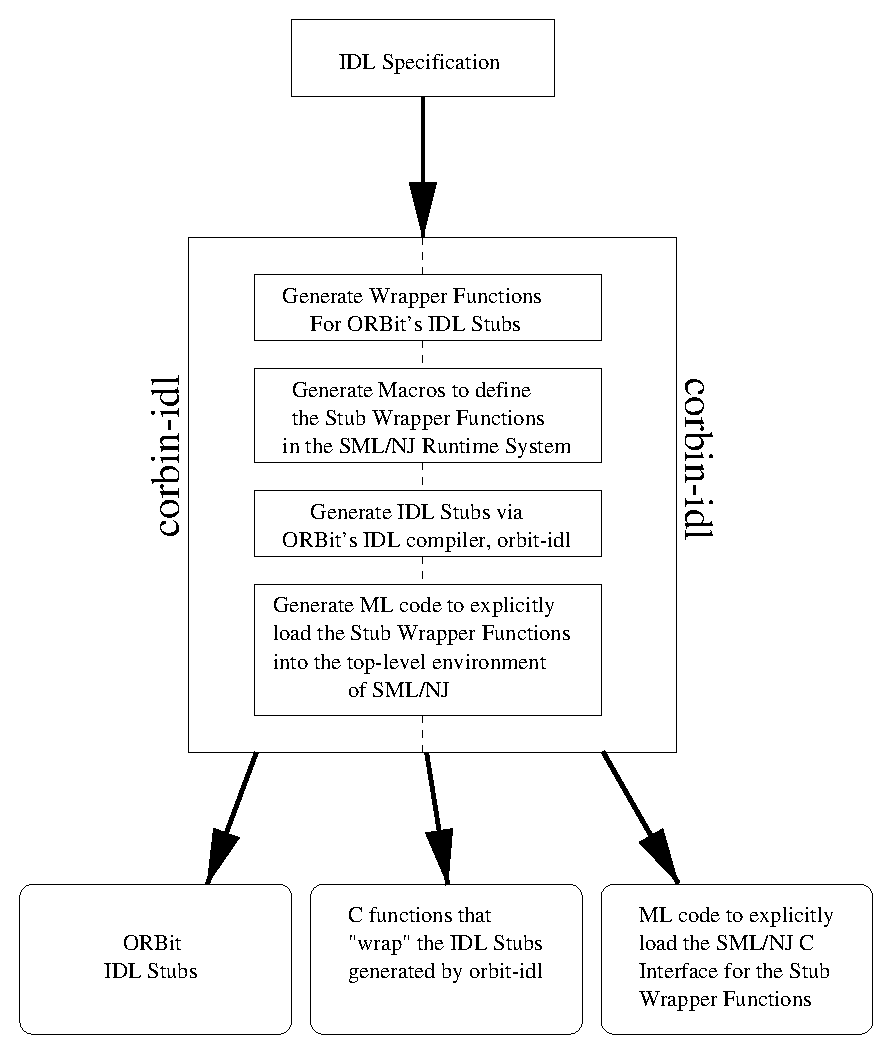
\psfig{file=Figures/corbinIDLStubs.eps}
\leavevmode
\caption{\em{Diagram of the corbin-idl stub generation process}.}
\figline
         \label{corbinIDLStubs}
\end{center}
\end{figure}

\subsection*{IDL skeletons}
\addcontentsline{toc}{subsection}{IDL skeletons} 

The first step in the corbin-idl skeleton generation process involves the 
generation of C function pointers.  These function pointers are used to 
retain references to ML functions.  When a request is received by 
ORBit to invoke an operation, the function pointers can be used 
to call the ML function that implements the requested operation. 
The function pointer generated for the foo object's bar operation is 
listed in figure \ref{CFunToML}.
\begin{figure*}[t]
\singlespace
\begin{verbatim}

  long (*CORBin_foo_bar_MLFn)(long );

\end{verbatim}
\doublespace
\caption {\em{C function pointer used to call the ML function that implements the foo object's bar operation}.}
\figline
        \label{CFunToML}
\end{figure*}

Once function pointers have been generated for all operations in the IDL
specification, corbin-idl generates C functions that are included in the 
SML/NJ runtime system so that the ML programmer can assign to these function 
pointers the address of the ML function that implements the corresponding 
operation. The C function generated by corbin-idl to save a pointer to 
the ML function that implements the foo object's bar operation is listed 
in figure \ref{CSaveMLPtr}.
\begin{figure*}[t]
\singlespace
\begin{verbatim}

  void CORBin_foo_bar_SetMLFn(long  (*f)(long ))
  {
       CORBin_foo_bar_MLFn = f;
  }

\end{verbatim}
\doublespace
\caption {\em{C function used to save a pointer to the ML function that implements the foo object's bar operation}.}
\figline
        \label{CSaveMLPtr}
\end{figure*}

Having generated the function pointer assignment functions, 
corbin-idl now generates C functions to {\em{callback}} the appropriate 
ML function.   
These functions are called when ORBit receives a request to invoke
an operation on an object.  So, when a request is received and this function 
is called, it simply passes the parameters of interest along to the function
implemented by the ML programmer.  The C function generated by corbin-idl 
to {\em{callback}} the ML function that implements the foo object's bar 
operation is shown in figure \ref{CCallBackToML}.
\begin{figure*}[t]
\singlespace
\begin{verbatim}

  static long
  impl_foo_bar(impl_POA_foo * servant , long x, 
               CORBA_Environment * ev)
  {
     return CORBin_foo_bar_MLFn(x);
  }

\end{verbatim}
\doublespace
\caption {\em{C function generated by corbin-idl that is called by ORBit when a client application invokes the bar operation on the foo object}.}
\figline
        \label{CCallBackToML}
\end{figure*}

Once corbin-idl has generated the necessary C functions for the IDL skeletons, 
it must generate C macros to explicitly define the functions that must be 
accessible from the SML/NJ runtime system.  Since the function pointer
assignment functions are the only functions that the ML programmer must be 
able to call explicitly, we only need to generate macros to define those 
functions.  The C macro generated by corbin-idl for the 
CORBin\_foo\_bar\_SetMLFn function is listed in figure \ref{CMLFnMacro}. 
\begin{figure*}[t]
\singlespace
\begin{verbatim}

     C_CALLS_CFUNC("CORBin_foo_bar_SetMLFn",
                    CORBin_foo_bar_SetMLFn, 
                    void , (long  (*f)(long )  ))

\end{verbatim}
\doublespace
\caption {\em{C Macro to explicitly define the CORBin\_foo\_bar\_SetMLFn function in the SML/NJ runtime system}.}
\figline
        \label{CMLFnMacro}
\end{figure*}
In order to produce C code to marshall and de-marshall parameters for the 
skeleton related functions generated by corbin-idl, orbit-idl is now executed. 

Just like the corbin-idl stub generation process, we must now generate 
ML code to explicitly load all of the necessary functions that have been 
generated into the top-level environment of SML/NJ.  Also, since 
the function pointer assignment functions are the only functions generated 
during this process that the ML programmer must have the ability to call, 
we are only concerned with them during this step.  First, we must generate
ML signatures for each of the applicable functions.  The ML signature 
generated for CORBin\_foo\_bar\_SetMLFn is listed in figure \ref{CFunToMLSig}.
\begin{figure*}[t]
\singlespace
\begin{verbatim}

     val CORBin_foo_bar_SetMLFn : (cdata list -> cdata) ->  unit

\end{verbatim}
\doublespace
\caption {\em{ML signature for the CORBin\_foo\_bar\_SetMLFn function}.}
\figline
        \label{CFunToMLSig}
\end{figure*}
Following the generation of signatures, corbin-idl generates value/function 
pairs for the appropriate functions.  
\pagebreak
Figure \ref{MLSetFnValFun} lists 
the ML code generated during this step for the CORBin\_foo\_bar\_SetMLFn
function.   
\begin{figure*}[t]
\singlespace
\begin{verbatim}

val CORBin_foo_bar_SetMLFn' =
     registerAutoFreeCFn("CORBin_foo_bar_SetMLFn", 
                         [CfunctionT([ClongT], ClongT)],CvoidT)
fun CORBin_foo_bar_SetMLFn f =
     let val  Cvoid  = 
              CORBin_foo_bar_SetMLFn' [Cfunction f] 
     in  
         ()
     end

\end{verbatim}
\doublespace
\caption {\em{ML value/function pair for the CORBin\_foo\_bar\_SetMLFn function}.}
\figline
        \label{MLSetFnValFun}
\end{figure*}
These key steps in the corbin-idl skeleton generation process are illustrated 
in figure \ref{corbinIDLSkels}. 
\begin{figure}
\begin{center}
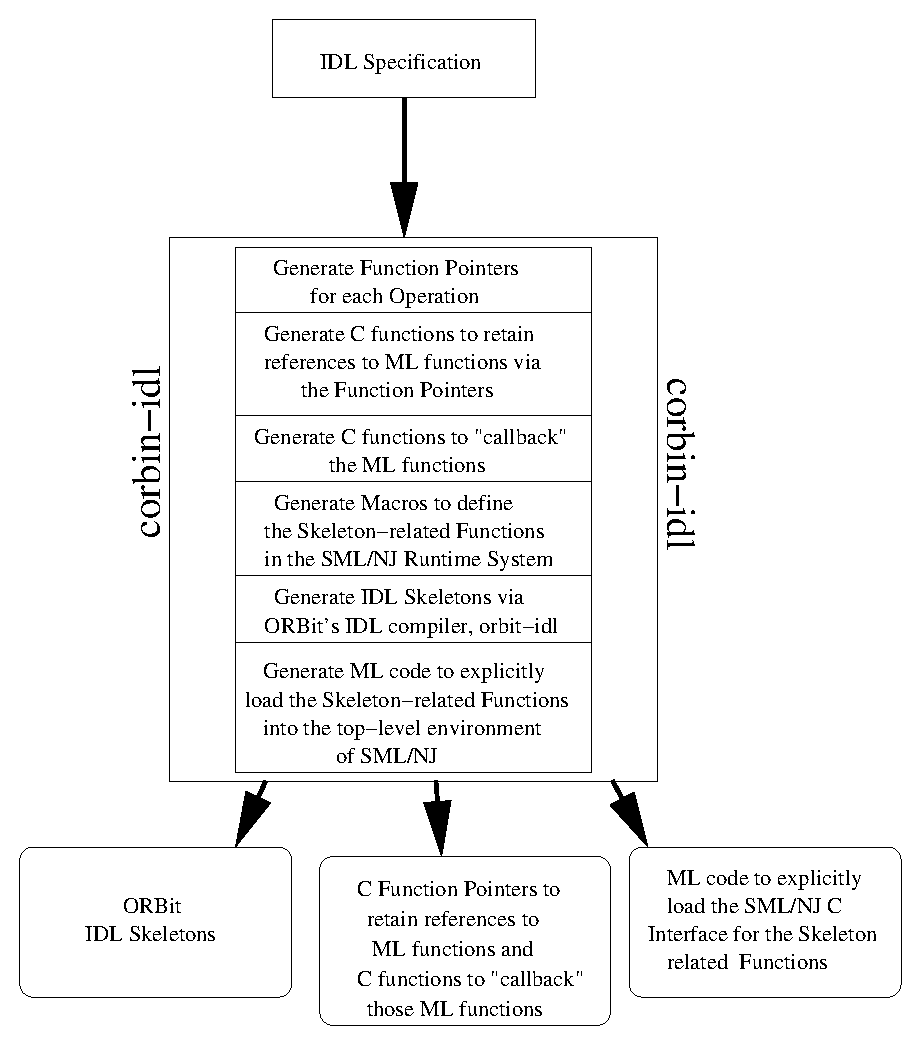
\psfig{file=Figures/corbinIDLSkels.eps}
\leavevmode
\caption{\em{Diagram of the corbin-idl skeleton generation process}.}
\figline
         \label{corbinIDLSkels}
\end{center}
\end{figure}

\newpage
\section*{\underline{The Library}}
\addcontentsline{toc}{section}{The Library}

The CORBin Library makes up the other half of the C ORB Interface System.
This library of C functions is combined with the SML/NJ runtime system in 
order to give ML programmers the ability to utilize ORBit's CORBA 
functionality.  This concept is illustrated in figure \ref{CORBinVisual}. 
\begin{figure}
\begin{center}
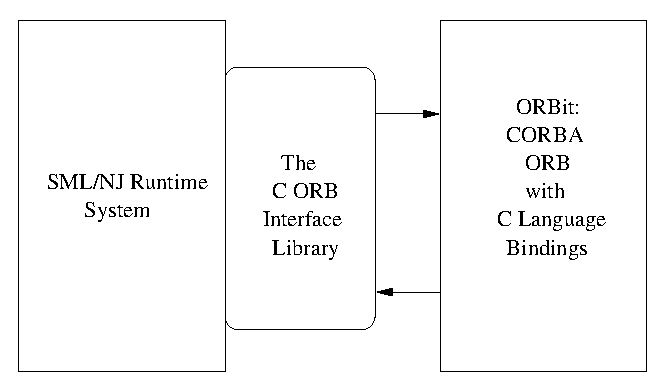
\psfig{file=Figures/CORBinVisual.eps}
\leavevmode
\caption{\em{The C ORB Interface Library}.}
\figline
         \label{CORBinVisual}
\end{center}
\end{figure}
The C functions in this library provide a standard interface 
to routines that already exist in ORBit.  They allow the ML programmer 
to use the most basic of ORBit's functionality and also the CORBA Name 
Service.  The basic routines that make up the CORBin Library are listed 
in figure \ref{CorbinLibrary}.  In addition to these basic routines, 
corbin-idl adds the necessary IDL stub and skeleton routines to this 
library when it processes IDL specifications.   
\begin{figure}
\begin{center}
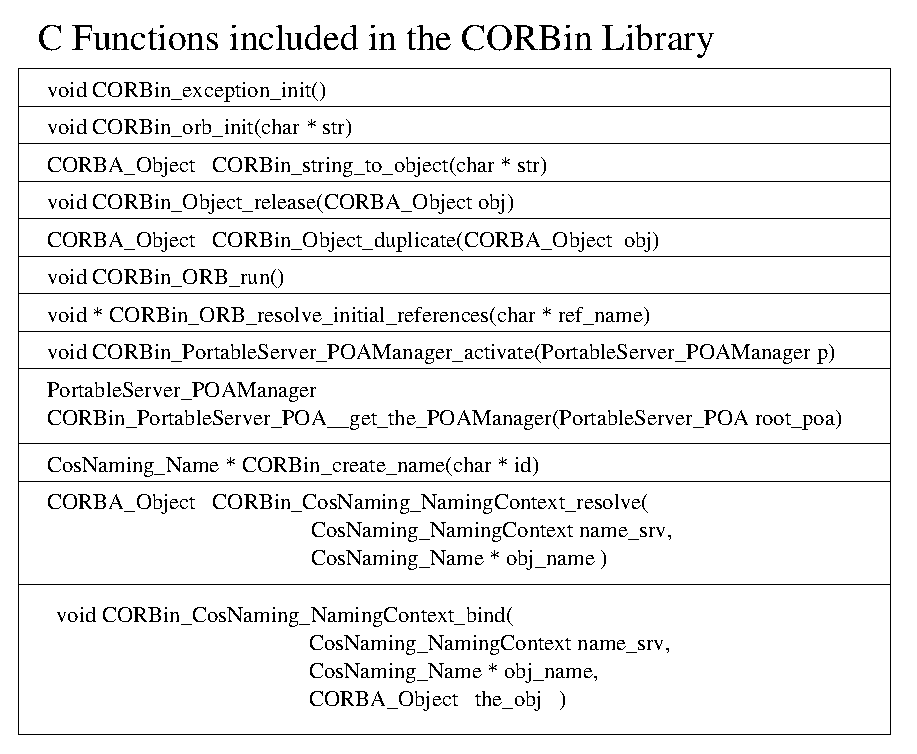
\psfig{file=Figures/CorbinLibrary.eps}
\leavevmode
\caption{\em{C Functions that make up the CORBin Library}.}
\figline
         \label{CorbinLibrary}
\end{center}
\end{figure}


